\subsection{Cross-validated results}
This paper demonstrates how CNN and ensemble models can be used to classify multiple cardiac abnormalities using 12-lead ECG-recordings. The cross-validated results show that the proposed ensemble model, using features from 12 leads, outperforms the other nine models on the development dataset from PhysioNet/CinC Challenge 2020. F1, F2, G2 and the PhysioNet/CinC Challenge Score was used to score the models. The 12-lead ensemble model were significantly better than all other models, measured on all four metrics.

The winner of PhysioNet/CinC Challenge 2020 reported a mean  cross-validated PhysioNet/CinC Challenge Score of $0.533\pm0.046$ SD \cite{natarajan_wide_nodate}, which was slightly better than the best score achieved in this study: $0.512\pm 0.006$. It is important to bear in mind that the cross-validated scores achieved on the development set, in this study, should be compared with caution to the reported scores on the PhysioNet/CinC Challenge 2020 hidden test set from other studies \cite{natarajan_wide_nodate,singstad_convolutional_nodate}. Even if some papers demonstrated good agreement between their cross-validated results, on the development set, and the results achieved on the hidden test set \cite{natarajan_wide_nodate}, the organizer reported that high-performing algorithms exhibited significant drops ($\approx 10\%$) in performance on the hidden test data \cite{alday_classification_2020}.

Surprisingly, the CNNs with the lowest complexity performed best compared to the rest of the CNNs. The Encoder model were significantly better in terms of F1, F2 and G2-score (figure \ref{fig:crossval_score}a-c), but closly follwed by FCN and FCN $||$ Gender\&Age when looking at the PhysioNet/CinC Challenge Score (Figure \ref{fig:crossval_score}d). Nevertheless, it is stated in \cite{singstad_convolutional_nodate} that the Encoder performed worse than FCN $||$ Gender\&Age, Encoder $||$ Gender\&Age, Encoder $||$ FCN + rule-based model and Encoder $||$ FCN $||$ Gender\&Age + rule-based model on a subset of the hidden test set. This observation emphasizes that one should be careful when comparing cross-validated scores with scores achieved on the hidden test set.

The FCN $||$ Encoder and the FCN $||$ Encoder $||$ Gender\&Age appeared to be unaffected by adding the rule-based model. No significant differences can be seen for any of the scoring methods in figure \ref{fig:crossval_score}. A possible explanation for this might be that the rule-based model allways agreed with the CNN-model and thus did not change the prediction. Another possible explanation for this is that the rule-based model failed to analyze the ECG and then did not make any prediction. One should keep in mind that these rule-based algorithm were really simple and therefore the these results should be interpreted with caution.

Another surprising aspect was that the ensemble model, using features from 2 leads, performed significantly better than all CNN models, using all 12 leads, on the PhysioNet Challenge Score (figure \ref{fig:crossval_score}d). However, it should be mentioned that the Encoder performed equally well on the F1, F2 and G2-score as seen in figure \ref{fig:crossval_score}a-c.

A possible limitation in this study is that the ECGs were not filtered before feeding them into the model or before extracting features with the ECG-featurizer. Some of the ECGs showed a lot of noise, like the ECG in figure \ref{fig:noisy_leadII}. Further studies are needed to determine if a filtered ECG signal would improve the performace of the models used in this study.

\begin{figure}[!hbp]
    \centering
    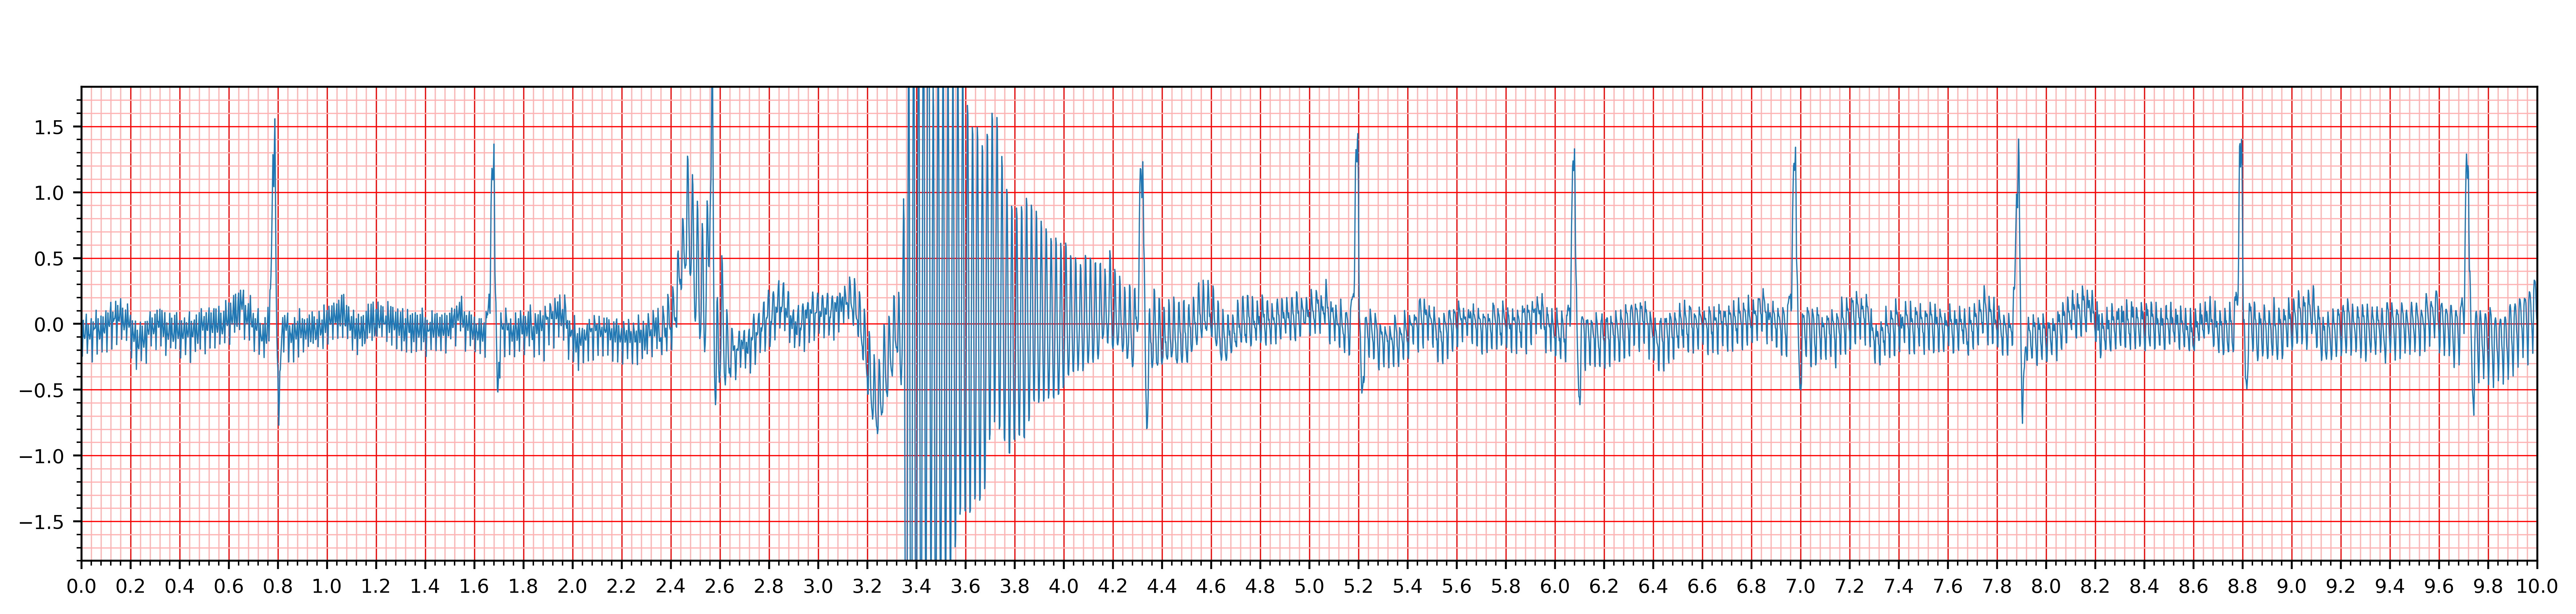
\includegraphics[width=.90\textwidth]{Figures/noisy_leadII.png}
    \caption{The figure shows a noisy ECG-signal from ECG Lead II}
    \label{fig:noisy_leadII}
\end{figure}


Limitation regarding LIME vs SHAP

Our findings emphasize the need to continue to develop explainability models for time series classifiers. 



The $84$ unscored diagnoses that were overlooked but still represented noise in the dataset.and did not represent any change in the 27-bit long label arra

It might be possible to uncover new features in the ECG that cardiologists should consider when interpreting ECG from athletes.